\documentclass[10pt]{article}
\usepackage[margin=0.73in]{geometry}
\usepackage{amsmath,amssymb,amsthm,mathtools}
\usepackage{graphicx}
\usepackage{microtype}
\usepackage{xcolor}
\usepackage[colorlinks=true,linkcolor=blue!50!black,citecolor=blue!50!black,urlcolor=blue!50!black]{hyperref}

\newtheorem{theorem}{Theorem}
\newtheorem{lemma}{Lemma}
\newcommand{\N}{\mathbb N}
\newcommand{\E}{\mathbb E}
\newcommand{\Q}{\mathcal Q}
\newcommand{\Sdom}{\mathcal S_1^+}
\setlength{\parindent}{0pt}
\setlength{\parskip}{4pt}

\title{The positive generator for reflection-symmetric small-step walks}
\author{Candidate partial result for arXiv:2012.08947}
\date{27 August 2026}

\begin{document}
\maketitle

\vspace{-1.2em}
\begin{center}
\fbox{\parbox{0.94\textwidth}{\textbf{Status.}
Candidate substantial partial result, likely valid, pending expert review.
The original conjecture remains open outside the family treated here.}}
\end{center}

\section*{Source question}

Hoang, Raschel and Tarrago construct a distinguished basis
$\{h_n\}_{n\geq1}$ of killed harmonic functions in the quarter plane.  Their
Conjecture~1 asks whether the first generator $h_1$ spans the unique positive
harmonic ray \cite[p.~9]{HRT}.

\begin{center}
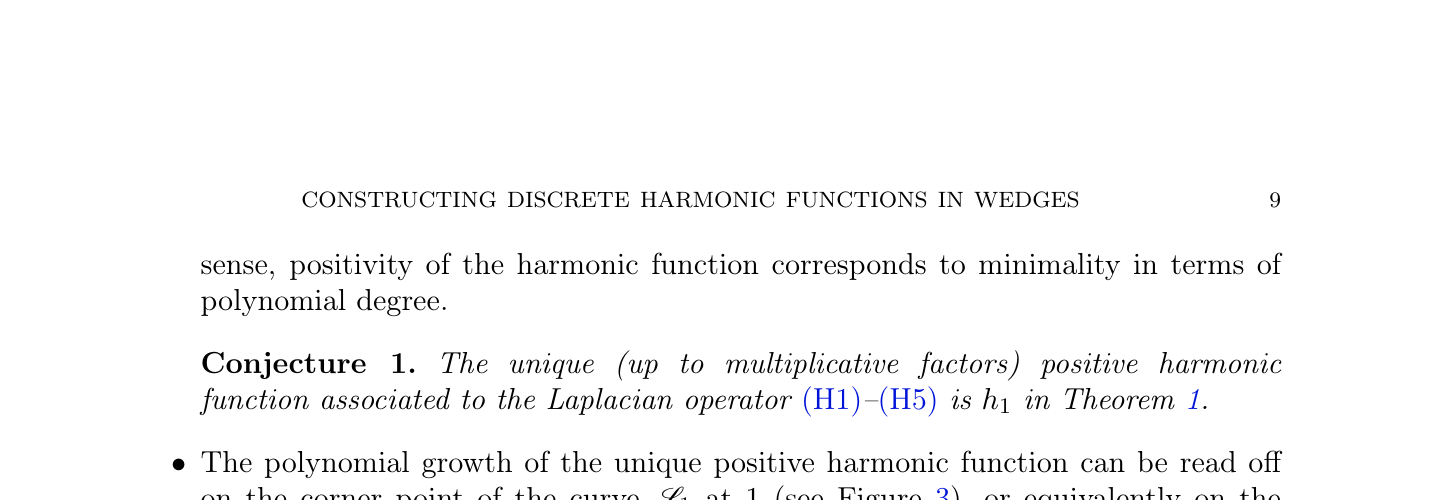
\includegraphics[width=0.91\textwidth]{figures/conjecture_1_crop.png}
\end{center}
\vspace{-0.7em}
\textbf{Transcription.} ``The unique (up to multiplicative factors) positive
harmonic function associated to the Laplacian operator (H1)--(H5) is $h_1$ in
Theorem 1.''

\section*{Definitions and result}

Put $\Q=\N^2=\{1,2,\ldots\}^2$ and kill the walk on leaving $\Q$.
Consider the square-symmetric small-step law
\begin{equation}\label{eq:law}
 p_{\pm1,0}=p_{0,\pm1}=\alpha,\qquad
 p_{\pm1,\pm1}=\beta,\qquad p_{0,0}=\gamma,
 \qquad 4\alpha+4\beta+\gamma=1,
\end{equation}
where $\alpha>0$ and $\beta,\gamma\geq0$; all unlisted probabilities vanish.
Thus the law is invariant under both coordinate reflections and coordinate
interchange.  The assumption $\alpha>0$ ensures irreducibility.

For the source kernel and generating functions we use
\begin{align*}
 K(x,y)&=xy-\sum_{k,\ell}p_{k,\ell}x^{1-k}y^{1-\ell},\\
 H(x,y)&=\sum_{i,j\geq1}h(i,j)x^{i-1}y^{j-1}.
\end{align*}

\begin{theorem}\label{thm:main}
For every law \eqref{eq:law}, the line spanned by the source generator $h_1$
contains the function
\[
 h(i,j)=ij\quad(i,j\geq1),\qquad h(i,j)=0\quad(i\leq0\ \hbox{or}\ j\leq0).
\]
Consequently $h_1$ spans the unique positive killed harmonic ray, so
Conjecture~1 of \cite{HRT} holds for the whole family \eqref{eq:law}.
This family contains the simple walk, the king walk, their mixtures, and all
lazy versions.
\end{theorem}

\section*{Proof Intuition}

Square symmetry kills exactly the three error terms in the one-step expansion
of $(i+X)(j+Y)$, so $ij$ is harmonic.  The less obvious task is to show that it
is the \emph{particular} harmonic function produced by the source's conformal
generator.  Here the generating function of $ij$ does that job for us: its
kernel equation isolates a rational function $\psi(x)$.  On the kernel curve,
that identity says $\operatorname{Re}\psi=0$.  The rational function has the
right double pole at the $\pi/2$ corner and no critical point in the kernel
domain, so it is precisely the source Riemann map up to its harmless positive
scale.  The source formula for $H_1$ then collapses to the generating function
of $ij$.

\section*{Proof}

Let $(X,Y)$ have law \eqref{eq:law}.  Reflection invariance gives
\[
 \E X=\E Y=0,
 \qquad
 \E(XY)=\beta-\beta-\beta+\beta=0.
\]
Since the jumps are small, a step from $\Q$ can hit an axis but cannot
overshoot it.  The zero extension of $h(i,j)=ij$ therefore agrees at every
possible endpoint with $(i+X)(j+Y)$, even when $i=1$ or $j=1$.  Hence
\[
 \E h(i+X,j+Y)
 =ij+i\E Y+j\E X+\E(XY)=ij.
\]
Thus $h$ is positive and killed harmonic, and
\begin{equation}\label{eq:H}
 H(x,y)=\frac1{(1-x)^2(1-y)^2},\qquad
 H(x,0)=\frac1{(1-x)^2},\qquad H(0,0)=1.
\end{equation}

The boundary pieces of the kernel are
\[
 K(x,0)=-\alpha x-\beta(x^2+1),\qquad K(0,0)=-\beta.
\]
Substituting \eqref{eq:H} in the source functional equation
\[
 KH=K(x,0)H(x,0)+K(0,y)H(0,y)-K(0,0)H(0,0)
\]
gives
\begin{equation}\label{eq:key}
 K(x,y)H(x,y)=-\frac{\psi(x)+\psi(y)}2,\qquad
 \psi(x)=\frac{\beta(x^2+1)+2(\alpha+\beta)x}{(1-x)^2}.
\end{equation}

\begin{lemma}\label{lem:psi}
The function $\psi$ in \eqref{eq:key} is, up to a positive multiplicative
constant allowed by the normalization, the conformal coordinate $\psi_1$ of
\cite{HRT} from the bounded kernel domain $\Sdom$ to the right half-plane.
\end{lemma}

\begin{proof}
For $x\in\partial\Sdom=\mathcal S_1$, the source construction supplies the
kernel pair $(x,\bar x)$.  Away from the corner $1$, setting $K(x,\bar x)=0$
in \eqref{eq:key} yields
\[
 \psi(x)+\psi(\bar x)=0.
\]
The coefficients of $\psi$ are real, so $\operatorname{Re}\psi(x)=0$ on
$\mathcal S_1\setminus\{1\}$.  Moreover,
\begin{equation}\label{eq:derivative}
 \psi'(x)=\frac{2(\alpha+2\beta)(x+1)}{(1-x)^3}.
\end{equation}
The Jordan domain $\Sdom$ lies in the unit disk.  Irreducibility excludes
$-1$ from its boundary (a unit-modulus kernel point other than $1$ would make
the walk periodic in the sense excluded by source hypothesis (H3)).  Thus
\eqref{eq:derivative} has no zero on $\overline{\Sdom}$.

Square symmetry also gives mixed covariance $\sigma_{12}=0$, so the corner
angle in \cite[(1.16)]{HRT} is $\theta=\pi/2$.  The sole singularity of $\psi$
on the boundary is
\[
 \psi(x)\sim\frac{2\alpha+4\beta}{(1-x)^2}\qquad(x\to1),
\]
exactly the order $\pi/\theta=2$ required at that corner.  Because $\psi'$
never vanishes, the zero set of $\operatorname{Re}\psi$ cannot acquire an
additional arc in $\Sdom$: such an arc cannot close (by the maximum
principle), cannot end in the interior, and cannot meet the smooth boundary
without locally coinciding with it.  At the only nonsmooth point, the double
pole and the right-angle corner supply exactly the two boundary arms.  Thus
$\operatorname{Re}\psi$ has constant sign in $\Sdom$.  It is positive because
$\psi(0)=\beta>0$ when $\beta>0$.

The map to $\mathcal H^+$ is proper: approaching the smooth boundary sends
$\psi$ to the imaginary axis, while approaching $1$ sends $|\psi|$ to
infinity.  Its degree is especially easy to count.  The equation
$\psi(x)=\beta$ reduces to $2(\alpha+2\beta)x=0$, so $0$ is its only finite
solution.  Hence the proper map has degree one.  When $\beta=0$, removing the
holding probability leaves the simple-walk kernel curve and $\psi$ is a
positive multiple of $x/(1-x)^2$; for every positive regular value its two
roots are reciprocal, with exactly one in the unit disk.  The degree is again
one.  Hence $\psi$ is conformal.  Uniqueness of the source Riemann map gives
$\psi_1=c\psi$ for some $c>0$ (with $c$ fixed by whichever of the source's
equivalent normalizations is used).
\end{proof}

For $n=1$, the source polynomial is $P_1(X)=X$, and Theorem~1 of \cite{HRT}
therefore gives
\[
 H_1(x,y)=\frac{\psi_1(x)+\psi_1(y)}{K(x,y)}.
\]
Using Lemma~\ref{lem:psi} and \eqref{eq:key},
\[
 H_1(x,y)=-2cH(x,y)
 =\frac{-2c}{(1-x)^2(1-y)^2}.
\]
Coefficient extraction yields $h_1(i,j)=-2cij$.  (The sign only records the
source Riemann-map normalization; the conjecture is stated up to nonzero
multiplicative factors.)  Finally, finite support supplies every moment needed
by the standard uniqueness theorem for the positive killed harmonic function
invoked immediately before Conjecture~1 in \cite{HRT}; see also
\cite{BMS}.  Hence the line spanned by $h_1$ is exactly the unique positive
ray.  This proves Theorem~\ref{thm:main}. \qed

\section*{Verification, limits, and novelty}

The moment computation, all three kernel boundary terms, the derivative
\eqref{eq:derivative}, and the coefficient extraction were checked separately.
The cases $\beta=0$ and $\gamma>0$ were audited explicitly: holding only
rescales the nontrivial harmonic equation.  The main expert-review point is
the degree-one argument in Lemma~\ref{lem:psi}; its boundary values, unique
pole, corner order, and absence of critical points are all displayed above.

The result does not cover asymmetric small-step laws or the source's walks
with larger negative jumps.  A bounded run-index and web/arXiv search on
27 August 2026 found the source's separate simple-walk and king-walk examples,
but no explicit statement for the full family \eqref{eq:law}.  Novelty is
therefore plausible but provisional, not certified by an exhaustive search.

\begin{thebibliography}{9}
\bibitem{HRT}
V. H. Hoang, K. Raschel and P. Tarrago,
\emph{Constructing discrete harmonic functions in wedges},
arXiv:2012.08947v2, 2023.

\bibitem{BMS}
A. Bouaziz, S. Mustapha and M. Sifi,
\emph{Discrete harmonic functions on an orthant in $\mathbb Z^d$},
Electron. Commun. Probab. \textbf{20} (2015), no. 52, 13 pp.
\end{thebibliography}

\end{document}
